\documentclass[aspectratio=169,9pt]{beamer}
\mode<presentation> 
\usepackage[utf8]{inputenc}
\usepackage{sansmathaccent} %Für equations
\usepackage{amsmath}
\usepackage{tikz}
\usepackage{multicol}
\usepackage{cancel}
\usepackage{relsize}
\usepackage{graphicx}
\usepackage[table]{xcolor}
\usepackage{fontawesome5}
\usepackage{enumitem}
\usepackage{setspace}
\usepackage[labelfont={bf},font={color=black!40,footnotesize},tablename={Tabelle},figurename={Abbildung}]{caption}
\usetikzlibrary{positioning, arrows.meta, calc}
\usefonttheme[onlymath]{serif}
%\makeatletter
%\makeatother

\usetikzlibrary{patterns, arrows.meta, calc}
\usepackage{pgfplots}
\pgfplotsset{compat=1.18}
\usetikzlibrary{intersections, pgfplots.fillbetween}\usetikzlibrary{intersections, pgfplots.fillbetween}
\rowcolors{2}{miugray!30}{miugray!10}

\usetheme{Madrid}  %% Themenwahl
\useoutertheme{split} % Alternatively: miniframes, infolines, split
%\useinnertheme{circles}


\setbeamertemplate{itemize item}{\color{miugray}$\blacksquare$}
\setbeamertemplate{itemize subitem}{\color{uniblau}$\bullet$}



%\newcommand{\metermilli}{\mskip3mu \text{mm}}
\newcommand{\cm}{\mskip3mu \text{cm}}
\newcommand{\m}{ \text{m}}
\newcommand{\lite}{ \text{l}}
\newcommand{\kg}{ \text{kg}}
\newcommand{\g}{ \text{g}}
\newcommand{\km}{ \text{km}}
\newcommand{\h}{ \text{h}}
\newcommand{\s}{ \text{s}}
\newcommand{\tonne}{ \text{t}}


\newcommand{\RA}{$\rightarrow$~}
\newcommand{\pp}{\par \vspace*{2mm}}
\newcommand{\ppbig}{\par \vspace*{4mm}}

\definecolor{miudiutex}{HTML}{1d2926}
\definecolor{miugray}{HTML}{b4cccf}
\definecolor{miugray2}{HTML}{4d7365}
\definecolor{white2}{HTML}{f5f7f8}
\definecolor{red}{HTML}{cf1f5c}
\definecolor{green}{HTML}{00A36C}
\definecolor{delphinidin}{HTML}{315794}
\definecolor{uniblau}{HTML}{004e9f}
\definecolor{unigelb}{HTML}{fcba00}
\definecolor{unigrau}{HTML}{909085}
\definecolor{pelargonidin}{HTML}{b33807}
\definecolor{cyanidin}{HTML}{ba0746}
\definecolor{paeonidin}{HTML}{d15ca6}
\definecolor{petunidin}{HTML}{b56fed}
\definecolor{malvidin}{HTML}{8a2d8c}

%\setbeamercolor{palette primary}{bg=pelargonidin!35,fg=white}
%\setbeamercolor{palette secondary}{bg=delphinidin!45,fg=white}
\setbeamercolor{palette primary}{bg=uniblau!70,fg=white}
\setbeamercolor{palette secondary}{bg=uniblau!45,fg=white}
\setbeamercolor{palette tertiary}{bg=unigelb!70,fg=unigrau}
\setbeamercolor{palette quaternary}{bg=miugray,fg=white}
\setbeamercolor{structure}{fg=black} % itemize, enumerate, etc
\setbeamercolor{section in toc}{fg=red} % TOC sections

\setbeamersize{text margin left=1cm,text margin right=1cm}


\useinnertheme{tcolorbox} 
\newcommand{\goodtk}[2]{
\begin{tcolorbox}[
	enhanced,
	colframe=uniblau!75,
	sharp corners,
	boxsep=5pt,
	title=\bfseries \sffamily #1,
	colback=white,
	coltitle=black,
	attach boxed title to top text left={yshift=-\tcboxedtitleheight/2},
	boxed title style={colback=white,colframe=white}
]
	#2
	\end{tcolorbox}
}
	
\newcommand{\antwort}[1]{
\begin{tcolorbox}[
	enhanced,
	colframe=unigrau!65,
	sharp corners,
	boxsep=1pt,
	colback=white,
	coltitle=black,
]
	#1
	\end{tcolorbox}
}


\title{6. Übung}
\author{PD Dr. Helene Loos}
\date{\today}

\begin{document}
%\maketitle
\small



\begin{frame}
\begin{center}

\LARGE Übung 6  \par \normalsize
Prozessbezogene Lebensmitteltechnologie
\end{center}
\small
\end{frame}









\begin{frame}

{\color{miugray}$\blacksquare ~$} \textbf{Kurze Wiederholung} \par \vspace*{2mm}
\pp
Charakteristische Länge $L$ oder $l$ für uns nur bei Berechnungen zu \textbf{Reynoldszahl} und \textbf{Nusseltzahl}
\ppbig

\begin{minipage}{.5\textwidth}

\textbf{Anwendungsbeispiele:}
\begin{itemize}
\item[$\cdot$] Rohrströmung \RA Innendurchmesser des Rohres
\item[$\cdot$] Umströmter Draht \RA Außendurchmesser
\item[$\cdot$] Kugel/Zylinder \RA Durchmesser
\item[$\cdot$] Platte/Hauswand \RA Länge in Strömungsrichtung
\end{itemize}
\end{minipage}%
\hspace*{4mm}
\begin{minipage}{.5\textwidth}

\antwort{

\textbf{Merkregel:} \pp 
Objekt rund? \RA Durchmesser \par 
Objekt flach? \RA Länge in Strömungsrichtung
}

\end{minipage}%
\pp
\begin{align*}
Re = \frac{\rho v \alert<1->{l}}{\eta} \\
Nu = \frac{\alpha \alert<1->{L}}{\lambda}
\end{align*}

\end{frame}


\begin{frame}

{\color{miugray}$\blacksquare ~$} \textbf{Kurze Wiederholung - Aufgabe 4} \par \vspace*{2mm}
\pp

\begin{minipage}{.5\textwidth}
a) Wie groß ist der \alert<2->{Wärmeübergangskoeffizient} innen, wenn Wasser
mit einer Geschwindigkeit von 0,5 m/s durch das Stahlrohr von
Aufgabe 3 fließt?
\pp
\begin{figure}
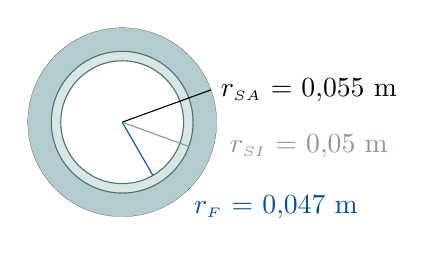
\begin{tikzpicture}[scale=0.6]
\draw[line width=0.01mm,fill=miugray] (0,0) circle (2cm);
\draw[miugray2,fill=miugray!50] (0,0) circle (1.5cm);
\draw[miugray2,fill=white] (0,0) circle (1.3cm);
\draw (0,0) to (20:2cm) node [right] {$r_\mathsmaller{{SA}}$ = 0,055 m};
\draw[miugray!75!black] (0,0) to (-20:1.5cm) node [right,xshift=4mm,yshift=0mm] {$r_\mathsmaller{{SI}}$ = 0,05 m};
\draw[uniblau] (0,0) to (-60:1.3cm) node [right,xshift=4mm,yshift=-4mm] {$r_\mathsmaller{{F}}$ = 0,047 m};
\end{tikzpicture}
\caption{Stahlrohr mit innerer Fouling-Schicht.}
\end{figure}
\end{minipage}%
\hspace*{4mm}
\begin{minipage}{.5\textwidth}
\antwort{
\begin{align*}
\uncover<3->{Nu &= \frac{\alpha \cdot l}{\lambda} \rightarrow \alpha = \frac{\alert<4->{Nu} \cdot \lambda}{l}} \\ \\
\uncover<5->{\text{Nu} &= \frac{(\frac{\alert<8->{\xi}}{8}) \cdot \text{\alert<7->{Re}} \cdot \text{\alert<6->{Pr}}}{1 + 12,7 \cdot (\frac{\alert<8->{\xi}}{8})^{\frac{1}{2}} \cdot (\text{\alert<6->{Pr}}^{\frac{2}{3}}-1)} \cdot \left[ 1 + (\frac{d}{l})^{\frac{2}{3}} \right]}
\end{align*}

}
\end{minipage}%

\end{frame}

\begin{frame}

{\color{miugray}$\blacksquare ~$} \textbf{Kurze Wiederholung - Aufgabe 4} \par \vspace*{2mm}
\pp
\begin{minipage}{.5\textwidth}
b) Wie ändert sich der Wärmestrom der Aufgabe 3 unter Berücksichtigung des Widerstands des inneren Wärmeübergangs? Berechnen Sie den Wärmestrom einmal mit und einmal ohne Fouling-Schicht
\pp
\begin{figure}
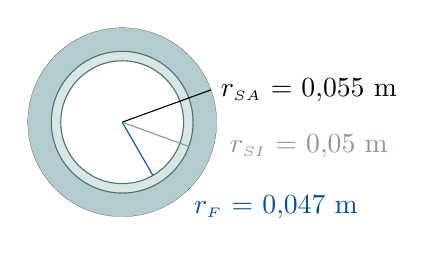
\begin{tikzpicture}[scale=0.6]
\draw[line width=0.01mm,fill=miugray] (0,0) circle (2cm);
\draw[miugray2,fill=miugray!50] (0,0) circle (1.5cm);
\draw[miugray2,fill=white] (0,0) circle (1.3cm);
\draw (0,0) to (20:2cm) node [right] {$r_\mathsmaller{{SA}}$ = 0,055 m};
\draw[miugray!75!black] (0,0) to (-20:1.5cm) node [right,xshift=4mm,yshift=0mm] {$r_\mathsmaller{{SI}}$ = 0,05 m};
\draw[uniblau] (0,0) to (-60:1.3cm) node [right,xshift=4mm,yshift=-4mm] {$r_\mathsmaller{{F}}$ = 0,047 m};
\end{tikzpicture}
\caption{Stahlrohr mit innerer Fouling-Schicht.}
\end{figure}
\end{minipage}%
\hspace*{4mm}
\begin{minipage}{.5\textwidth}
\antwort{
Stationäre (zeitlich unveränderliche) Wärmeleitung durch Rohr mit mehreren Schichten:
\large
\begin{align*}
\dot{Q} &= \frac{2 \pi \cdot l \cdot \Delta T }{\sum \frac{\ln(\frac{r_{a_n}}{r_{i_n}})}{\lambda_n}}\\[0.2cm]
		&= \frac{2 \pi \cdot l \cdot \Delta T }{\frac{\ln (\frac{r_{SI}}{r_{F}})}{\lambda_F} + \frac{\ln (\frac{r_{SA}}{r_{SI}})}{\lambda_S}}
\end{align*}

}
\end{minipage}%

\end{frame}

%\begin{frame}
%
%\begin{center}
%\LARGE Logarithmus \par 
%\large - Rechenregeln - 
%\end{center}
%
%\end{frame}


\begin{frame}

{\color{miugray}$\blacksquare ~$} \textbf{Kurze Wiederholung - Logarithmusregeln} \par \vspace*{2mm}
\pp
\Large

\begin{align*}
\log_x \left( u\cdot v \right) &= \log_x(u) + \log_x(v) \\ 
\log_x \left( \frac{u}{v} \right) &= \log_x(u) - \log_x(v) \\ 
\log_x \left( u^v \right) &= v \cdot log_x(u)
\end{align*}

\end{frame}



\begin{frame}

\begin{center}
\LARGE Übungsblatt 6
\end{center}

\end{frame}



\begin{frame}
\begin{minipage}{.5\textwidth}


{\color{miugray}$\blacksquare ~$} \textbf{Aufgabe 1} \par \vspace*{2mm}
Beim Erhitzen einer Sporensuspension bei 112 °C werden folgende Sporenzahlen nach unterschiedlichen Erhitzungszeiten festgestellt:


\pp
\begin{center}\begin{tabular}{rr}
\rowcolor{miugray}
Zeit [min] & Sporenzahl \\ \hline
0 &1.000.000 \\
4 &110.000 \\
8 &12.000 \\
12 &1.200 \\
\end{tabular}\end{center}

Bestimmen Sie den D-Wert sowohl 
\begin{enumerate}[label=\alph*)]
\item mittels semi-logarithmischer graphischer Auftragung (nutzen Sie dafür den vorgegebenen Graphen) 
\item rechnerisch
\end{enumerate}

\end{minipage}%
\hspace*{4mm}
\begin{minipage}{.5\textwidth}
\antwort{
\resizebox{\textwidth}{!}{
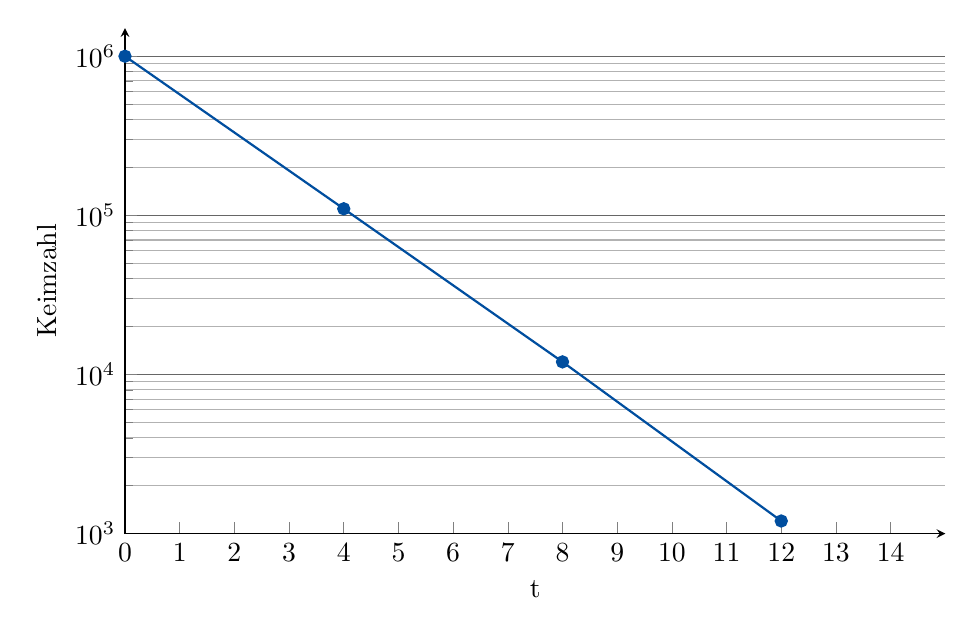
\begin{tikzpicture}
    \begin{semilogyaxis}[
        width=12cm,
        height=8cm,
        xmin=0, xmax=15,       % Grenzen der X-Achse
        ymin=1000, ymax=1500000,    % Grenzen der Y-Achse (3 Dekaden: 10^0 bis 10^3)
        enlarge y limits={upper, value=0.05},
        axis lines=left,      % Achsenlinien nur links und unten
		ymajorgrids=true,     % NUR horizontale Haupt-Gitterlinien zeichnen
        yminorgrids=true,     % NUR horizontale Zwischen-Gitterlinien zeichnen
        major grid style={black!60, thin}, % Stil der Haupt-Gitterlinien (1, 10, 100...)
        minor grid style={black!30, thin}, % Stil der Zwischen-Gitterlinien (2, 3, 4...)
        minor y tick num=8,   % 8 Zwischenstriche pro Dekade
        xtick={0,1,2,3,4,5,6,7,8,9,10,11,12,13,14},
%        xticklabels={\empty}, % Versteckt die X-Achsen-Zahlen (wie im Bild)
%        yticklabels={\empty}, % Versteckt die Y-Achsen-Zahlen (wie im Bild)
        tick align=inside,   % Achsenstriche zeigen nach außen
        ylabel=Keimzahl,
        xlabel=t,
%        axis background/.style={fill=miugray!50}
    ]
%\addplot[color=blue, very thick, domain=0:7, samples=100] {1.5^x};
    % --- Hier kannst du deinen Graphen einfügen ---
    % Beispiel:

     \only<2->{\addplot[color=uniblau, thick, mark=*] coordinates {(0,1000000) (4, 110000) (8, 12000) (12, 1200)};}


    
    \end{semilogyaxis}
\end{tikzpicture}
}


\begin{align*}
\uncover<3->{D_{1\rightarrow 2} &= \frac{4 ~\text{min}}{\log (\frac{10^6}{1,1 \cdot 10^5})} &= 4,17 ~\text{min}\\}
\uncover<4->{D_{ges} &= \frac{12 ~\text{min} }{\log (\frac{10^6}{1,2 \cdot 10^3})} &= 4,11 ~\text{min}}
\end{align*}
}
\end{minipage}%

\end{frame}



\begin{frame}



\begin{minipage}{.5\textwidth}


{\color{miugray}$\blacksquare ~$} \textbf{Aufgabe 2} \par \vspace*{2mm}


Für eine Sporensuspension wurden folgende D-Werte bestimmt:
\begin{center}\begin{tabular}{rr}
\rowcolor{miugray}
Temperatur [°C] & D-Wert [min] \\ \hline
104 &27,5 \\
107 &14,5 \\
110 &7,5 \\
113 &4,0 \\
116 &2,2 \\

\end{tabular}\end{center}
\pp


Bestimmen Sie den z-Wert
\begin{enumerate}[label=\alph*)]
\item mittels semi-logarithmischer graphischer Auftragung (nutzen Sie dafür den vorgegebenen Graphen) 
\item rechnerisch
\end{enumerate}
\end{minipage}%
\hspace*{4mm}
\begin{minipage}{.5\textwidth}



\antwort{
\resizebox{\textwidth}{!}{
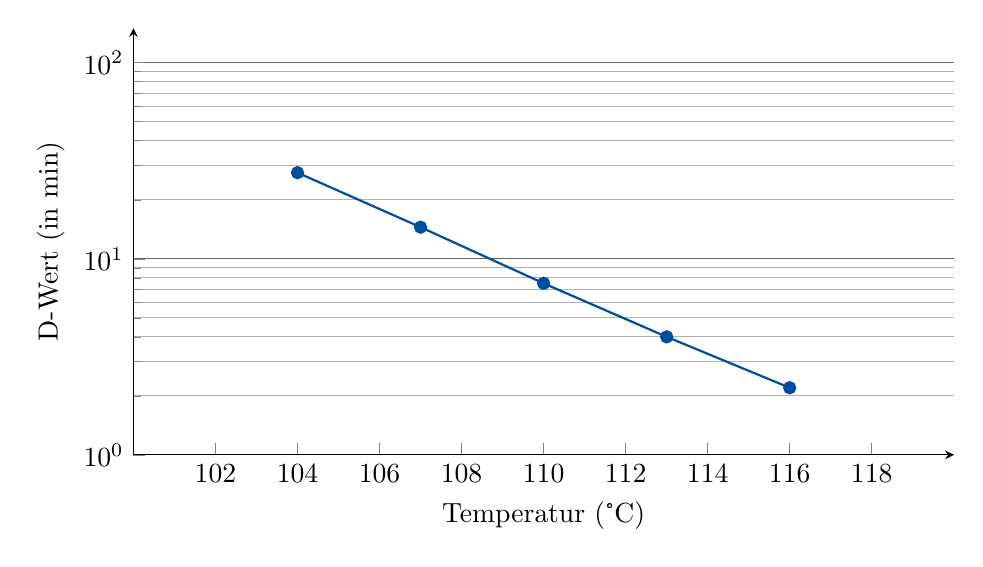
\begin{tikzpicture}
    \begin{semilogyaxis}[
        width=12cm,
        height=7cm,
        xmin=100, xmax=120,       % Grenzen der X-Achse
        ymin=1, ymax=150,    % Grenzen der Y-Achse (3 Dekaden: 10^0 bis 10^3)
        enlarge y limits={upper, value=0.05},
        axis lines=left,      % Achsenlinien nur links und unten
		ymajorgrids=true,     % NUR horizontale Haupt-Gitterlinien zeichnen
        yminorgrids=true,     % NUR horizontale Zwischen-Gitterlinien zeichnen
        major grid style={black!60, thin}, % Stil der Haupt-Gitterlinien (1, 10, 100...)
        minor grid style={black!30, thin}, % Stil der Zwischen-Gitterlinien (2, 3, 4...)
        minor y tick num=8,   % 8 Zwischenstriche pro Dekade
        xtick={102,104,106,108,110,112,114,116,118},
%        xticklabels={\empty}, % Versteckt die X-Achsen-Zahlen (wie im Bild)
%        yticklabels={\empty}, % Versteckt die Y-Achsen-Zahlen (wie im Bild)
        tick align=inside,   % Achsenstriche zeigen nach außen
        ylabel=D-Wert (in min),
        xlabel=Temperatur (°C)
    ]
    


\uncover<2->{\addplot[color=uniblau, thick, mark=*] coordinates {(104,27.5) (107,14.5) (110,7.5) (113, 4) (116,2.2)};}



    
    \end{semilogyaxis}
\end{tikzpicture}
}


\uncover<3->{
\begin{align*}
z &= \frac{T_2 - T_1}{\log(D_1) - \log (D_2)} \\
z &= \frac{107 - 104}{\log(27,5) - \log (14,5)} = 10,79 \\
z &= \frac{116 - 104}{\log(27,5) - \log (2,2)} = 10,93 \\
\end{align*}
}
}

\end{minipage}%

\end{frame}











\begin{frame}

{\color{miugray}$\blacksquare ~$} \textbf{Andwendung des z-Wertes in der Praxis} \par \vspace*{2mm}

\begin{figure}

\resizebox{.6\textwidth}{!}{
\begin{tikzpicture}[font=\sffamily\small]

\begin{semilogyaxis}[
    width=12cm, height=10cm,
    xmin=100, xmax=155,
    ymin=1, ymax=6000,
    axis lines=left,
    xlabel={Temperatur T, \textdegree C},
    ylabel={Zeit, s},
    % Positionierung der Achsenbeschriftungen anpassen
%    every axis x label/.style={at={(ticklabel* cs:0.5)}, anchor=north, yshift=-0.2cm},
%    every axis y label/.style={at={(0,1.05)}, anchor=south west, rotate=-90},
    % Ticks konfigurieren
    log ticks with fixed point,
    ytick={1,2,5,10,20,50,100,200,500,1000,2000,5000},
    xtick={90,100,110,120,130,140},
    tick align=inside,
    major tick length=4pt,
%    clip=false % Erlaubt das Zeichnen von Elementen leicht ausserhalb des Grids
]

% ==========================================
% KURVEN (berechnet nach der z-Wert Formel)
% ==========================================


% 40% Verlust (Grün): z=27, angenommener Referenzpunkt ~15s bei 135 °C
%\addplot [domain=90:143, miugray, line width=1.2pt] {15 * 10^((135 - x)/27)};

% 10% Verlust (Grün): z=27, angenommener Referenzpunkt ~3.56s bei 135 °C
\addplot [name path=neua,domain=132:150, white, line width=1.2pt] {3.56 * 10^((135 - x)/27)};
\addplot [name path=A,domain=100:150, miugray, line width=1.2pt] {3.56 * 10^((135 - x)/27)};


% F-Wert (Magenta): z=10, Startpunkt 60s bei 121.1 °C

\addplot [name path=neub,domain=132:143, white, line width=1.2pt] {60 * 10^((121.1 - x)/10)};
\addplot [name path=B,domain=102:143, uniblau, line width=1.2pt] {60 * 10^((121.1 - x)/10)};


\only<2->{
 \addplot[fill=uniblau,opacity=0.2]fill between[of=neua and neub,
% soft clip = {domain=150:132}
 ];}
% ==========================================
% DATENPUNKTE (Kreuze und Punkte)
% ==========================================
\addplot [only marks, mark=x, thick, uniblau, mark size=3pt] coordinates {
    (111.1, 600) 
    (121.1, 60)
};

%\addplot [only marks, mark=*, black, mark size=1.2pt] coordinates {
%    (110, 126) (135, 15)   % Punkte auf der 40% Linie
%    (110, 30)  (135, 3.56) % Punkte auf der 10% Linie
%};


% ==========================================
% BESCHRIFTUNGEN & ANNOTATIONEN
% ==========================================




% Verlust-Beschriftungen (Grün)
%\node[miugray, right, align=left] at (axis cs:92, 350) {\textbf{40 \%}\\\textbf{Verlust}};
\node[miugray2, right, align=left] at (axis cs:102, 100) {Kochgeschmack, \\ z = 27};
%\node[miugray, right] at (axis cs:100, 110) {\textbf{z = 27}};

% Optimaler Bereich & Kreis unten rechts
%\node[circle, fill=unigelb, minimum size=12pt, inner sep=0] at (axis cs:142, 1.4) {};
%\node[black, right] at (axis cs:139, 2.5) {140 \textdegree C $\sim$1,5 s};

\only<3->{\node[align=right, font=\footnotesize] (opt) at (axis cs:145, 20) {optimaler\\Bereich: \\ 140 \textdegree C $\sim$1,5 s};
\draw[-{Stealth[length=2.5mm, width=2mm]}] (opt) -- (axis cs:140, 1.5);}




% z- und F-Werte (Magenta)
%\node[uniblau, right] at (axis cs:119, 120) {z = 10};
\node[uniblau, right,align=left] at (axis cs:122.5, 100) {Sterilisation, \\ F = 1 min, z = 10, \\ T= 121,1 \textdegree C};


% "übersterilisiert" + Pfeil
\node[miugray!70, right, font=\bfseries] at (axis cs:120, 500) {übersterilisiert};
\draw[-{Stealth[length=3mm, width=2.5mm]}, miugray!70, thick] (axis cs:114, 350) -- (axis cs:132, 350);

\end{semilogyaxis}
\end{tikzpicture}
}




\caption{Ermittlung eines Temperatur-Zeit-Punktes unter Sicherheits- und Qualitätsaspekten (Muschiolik 2013)}
\end{figure}



\end{frame}


\begin{frame}
\begin{minipage}{.5\textwidth}


{\color{miugray}$\blacksquare ~$} \textbf{Aufgabe 3} \par \vspace*{2mm}


In einem Lebensmittel liegt die Anfangskeimzahl bei 1.000 Sporen pro Gramm. Es wird ein 12D-Konzept angewandt. Das Lebensmittel wird in 500 g-Packungen abgefüllt. 
\pp
In wie vielen Packungen ist nach der Erhitzung theoretisch noch eine Spore enthalten?




\end{minipage}%
\hspace*{4mm}
\begin{minipage}{.5\textwidth}
\antwort{
\uncover<2->{
Sporen pro Gramm:}
\uncover<3->{
\begin{align*}
1000 ~(\text{Sporen} /\text{g}) \cdot 10^{-12} = 10^{-9} ~(\text{Sporen} /\text{g})
\end{align*}
}
\uncover<4->{
Sporen pro 500 g - Packung:}
\uncover<5->{
\begin{align*}
10^{-9} \cdot 500 ~\text{g} = \frac{1}{2.000.000}
\end{align*}
}
\uncover<6->{
In einer von 2 Millionen Packungen ist noch eine Spore enthalten.
}
}
\end{minipage}%
\end{frame}




\begin{frame}
\begin{minipage}{.5\textwidth}


{\color{miugray}$\blacksquare ~$} \textbf{Aufgabe 4} \par \vspace*{2mm}


Die Anfangskeimbelastung liegt bei 10.000 Sporen pro Konserve. Es wird 50 min lang bei
113°C erhitzt. Der D-Wert liegt bei dieser Temperatur bei 4 min. 
\pp 
Wie hoch ist das Risiko, dass eine Packung eine Spore enthält?
\end{minipage}%
\hspace*{4mm}
\begin{minipage}{.5\textwidth}




\antwort{
\uncover<2->{
Formel aus Food Processing Handbook, S.35:
\begin{align}
\frac{\text{Heating Time}}{D_T} &= \log(\frac{N_0}{N}) 
\end{align}}
\uncover<3->{
Zunächst potenzieren wir um den Logarithmus umstellen zu können:
\begin{align*}
10^{\frac{\text{Heating Time}}{D_T}} &= \frac{N_0}{N} \\
N &= \frac{N_0}{10^{\frac{\text{Heating Time}}{D_T}}}
\end{align*}
}
\uncover<4->{
Werte einsetzen:
\begin{align*}
N &= \frac{10.000}{10^{\frac{\text{50 ~\text{min}}}{4 ~\text{min}}}} \\
 &= 3,16 \cdot 10^{-9}
\end{align*}
}
\uncover<5->{
Anzahl der Konserven, die geöffnet werden müssen um eine Spore zu finden:
\begin{align*}
\frac{1}{3,16 \cdot 10^{-9}} = 3,16 \cdot 10^{8}
\end{align*}
}
}
\end{minipage}%
\end{frame}




\begin{frame}
\begin{minipage}{.5\textwidth}


{\color{miugray}$\blacksquare ~$} \textbf{Aufgabe 5} \par \vspace*{2mm}


Wie lange muss erhitzt werden, um bei T = 75 °C einen Endkeimgehalt bzgl.
\textit{Streptococcus spp.} von 10$^{-3}$ pro Behältnis zu erreichen?
\par 

Konserveninhalt: 450 g \par 
Anfangskeimgehalt: 10$^2$/g \par 
D$_T^{Z}$ = D$_{80 ~\text{°C}}^{8,5 ~\text{°C}}$ = 0,5 min \par 



\end{minipage}%
\hspace*{4mm}
\begin{minipage}{.5\textwidth}
\antwort{
\uncover<2->{
D-Wert der neuen Temperatur ausrechnen:}
\uncover<3->{
\begin{align*}
D_1 &= D_2 \cdot 10^{\frac{T_2-T_1}{z}} \\
D_1 &= 0,5 ~\text{min}  \cdot 10^{\frac{80-75}{8,5}} \\
	&= 1,94
\end{align*}
}

\uncover<4->{
Anfangskeimgehalt einer 450 g-Konserve: }
\uncover<5->{
\begin{align*}
10^2 \cdot 450 = 45.000 
\end{align*}
}
\uncover<6->{ 
Zeit die nötig ist, um auf 10$^{-3}$ Sporen pro Behältnis zu reduzieren:}
\begin{align*}
\uncover<7->{
\text{Heating Time} &= D_T \cdot \log(\frac{N_0}{N}) \\}
\uncover<8->{\text{Heating Time} &= 1,94 \cdot \log(\frac{45.000}{10^{-3}}) \\
 &= 14,85 ~ \text{min}}
\end{align*}

}
\end{minipage}%


\end{frame}





\begin{frame}

\begin{minipage}{.4\textwidth}


{\color{miugray}$\blacksquare ~$} \textbf{Aufgabe 6} \par \vspace*{2mm}


In der folgenden Tabelle fehlen einige Angaben. Bitte füllen Sie diese Lücken aus. Nehmen Sie an, dass es sich hierbei nur um eine Reaktion handelt, sodass die Spalten
zueinander in einer Beziehung stehen. \par 





\end{minipage}%
\hspace*{4mm}
\begin{minipage}{.6\textwidth}


%\antwort{

\begin{spacing}{1.5}
\resizebox{\textwidth}{!}{
\begin{tabular}{lll}
\hline
\textbf{D-Wert} & \textbf{Temperatur} & \textbf{Zeit} \\
\hline
D$_{80\text{°C}}^{5 \text{°C}}$ = 0,5 min & T = 80 °C & t = 0,5 min \\
%\hline
D$_{70\text{°C}}^{5 \text{°C}}$ = 50 min & T = 70°C  & t = 50 min \\
%\hline
D$_{85\text{°C}}^{5 \text{°C}}$ = 0,05 min & T = 85 °C & t = 0,05 min \\
%\hline
D$_{100\text{°C}}^{5 \text{°C}}$ = 0,00005 min & T = 100°C &t = 0,00005 min \\
\hline
\end{tabular}

}
\end{spacing}

%}

\begin{align*}
T_2 = \log \left( \frac{D_1}{D_2} \right) \cdot z + T_1
\end{align*}

\end{minipage}%


\end{frame}









\begin{frame}

\begin{minipage}{.5\textwidth}


{\color{miugray}$\blacksquare ~$} \textbf{Aufgabe 7} \par \vspace*{2mm}
Sie haben für Ihren Erhitzungsprozess einen D-Wert von D$_{121,1}$ = 3 min gegeben. Wie sieht
der D-Wert bei einer Temperatur von 112 °C aus, wenn ein z-Wert von 10 °C gegeben ist?



\end{minipage}%
\hspace*{4mm}
\begin{minipage}{.5\textwidth}
\antwort{
\begin{align*}
D_1 &= D_2 \cdot 10^{\frac{T_2-T_1}{z}} \\
\uncover<2->{D_1 &= 3 \cdot 10^{\frac{121,1-112}{10}} \\
 &= 24,38 ~\text{min}}
\end{align*}
}
\end{minipage}%


\end{frame}




\end{document}
